\section{Общая для всех вариантов программа}

\subsection{Исследуемая программа}

Исходный текст исследуемой программы представлен на листинге \ref{lst:test_s}.
\begin{lstinputlisting}[
	label={lst:test_s},
	caption={Исходный текст общей программы},
	]{../riscv-lab/src/test.s}
\end{lstinputlisting}
\newpage

Дизассемблерный листинг исследуемой программы представлен на листинге \ref{lst:test_disasm}.
\begin{lstinputlisting}[
	label={lst:test_disasm},
	caption={Дизассемблерный листинг общей программы},
	]{../riscv-lab/src/test_disasm.s}
\end{lstinputlisting}
\newpage

Можно сказать, что данная программа эквивалентна псевдокоду на языке C, представленному на листинге \ref{lst:test_c}.
\begin{lstinputlisting}[
	label={lst:test_c},
	language=C,
	caption={Псевдокод на языке С},
	]{../riscv-lab/src/test.c}
\end{lstinputlisting}
\newpage


\subsection{Результаты исследования программы}

Скриншот, полученный в ходе выполнения задания №2 (получить снимок экрана, содержащий временную диаграмму выполнения стадий выборки и диспетчеризации команды с адресом 80000020 на первой итерации) представлен на рисунке \ref{fig:task280000020}.

\begin{figure}
	\centering
	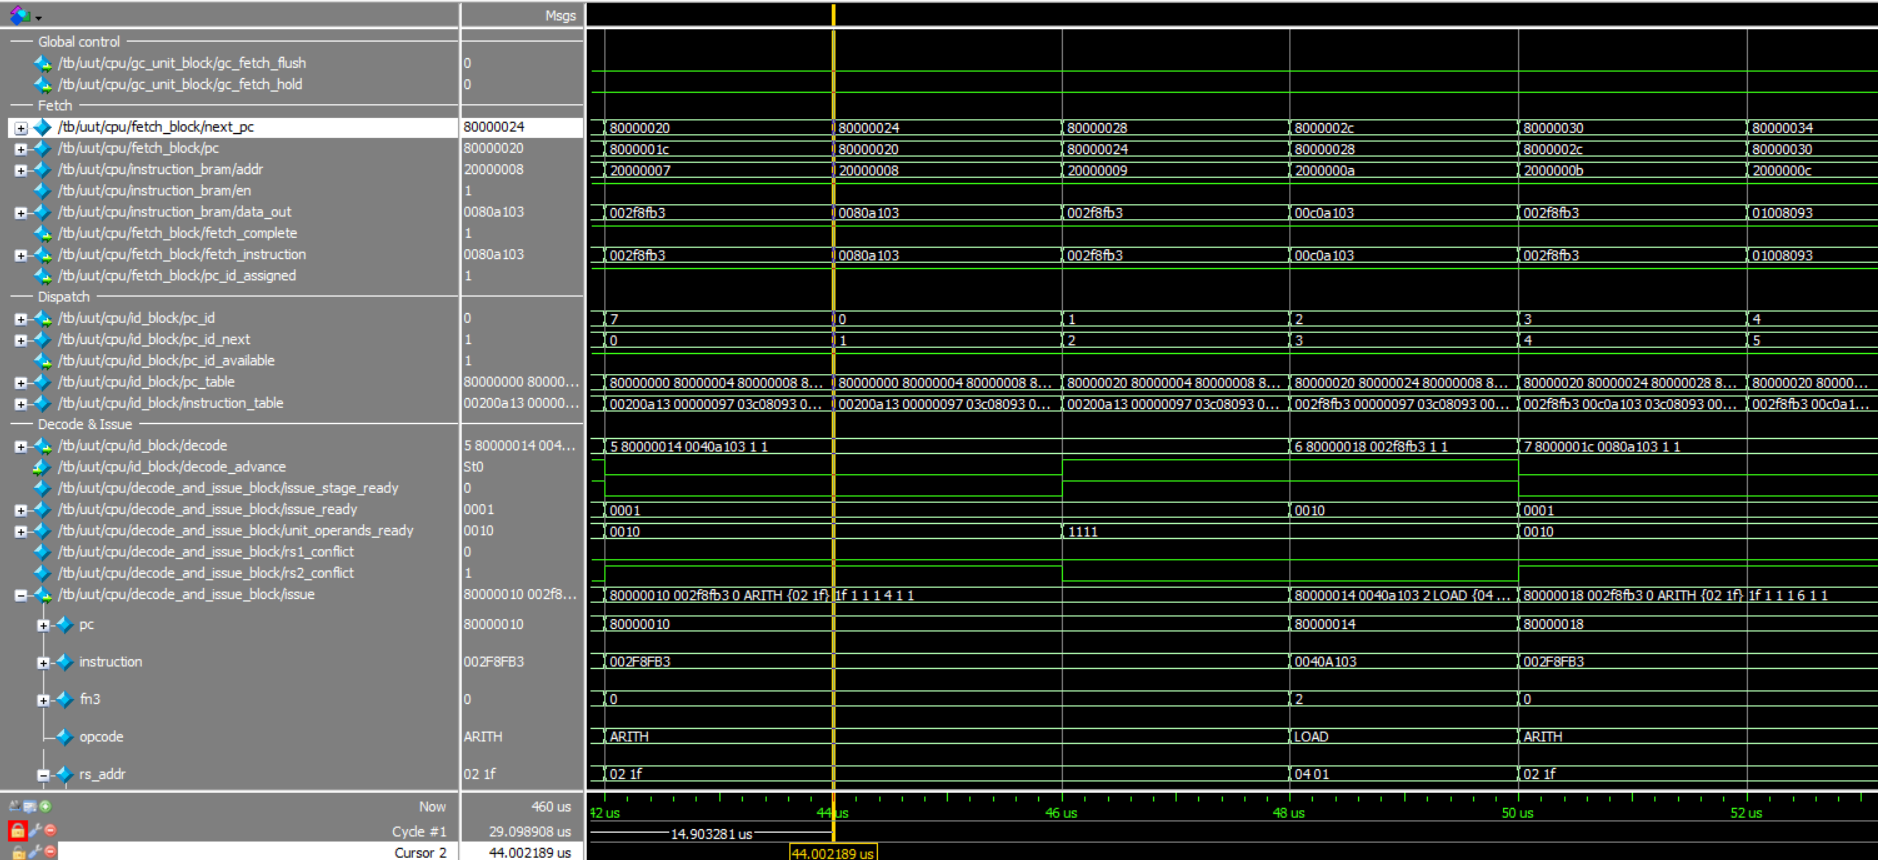
\includegraphics[width=1\linewidth]{../images/task2_80000020}
	\caption{Временная диаграмма выполнения стадий выборки и диспетчеризации}
	\label{fig:task280000020}
\end{figure}

Скриншот, полученный в ходе выполнения задания №3 (получить снимок экрана, содержащий временную диаграмму выполнения стадии декодирования и планирования на выполнение команды с адресом 8000002с на первой итерации) представлен на рисунке \ref{fig:task38000002c}.

\begin{figure}
	\centering
	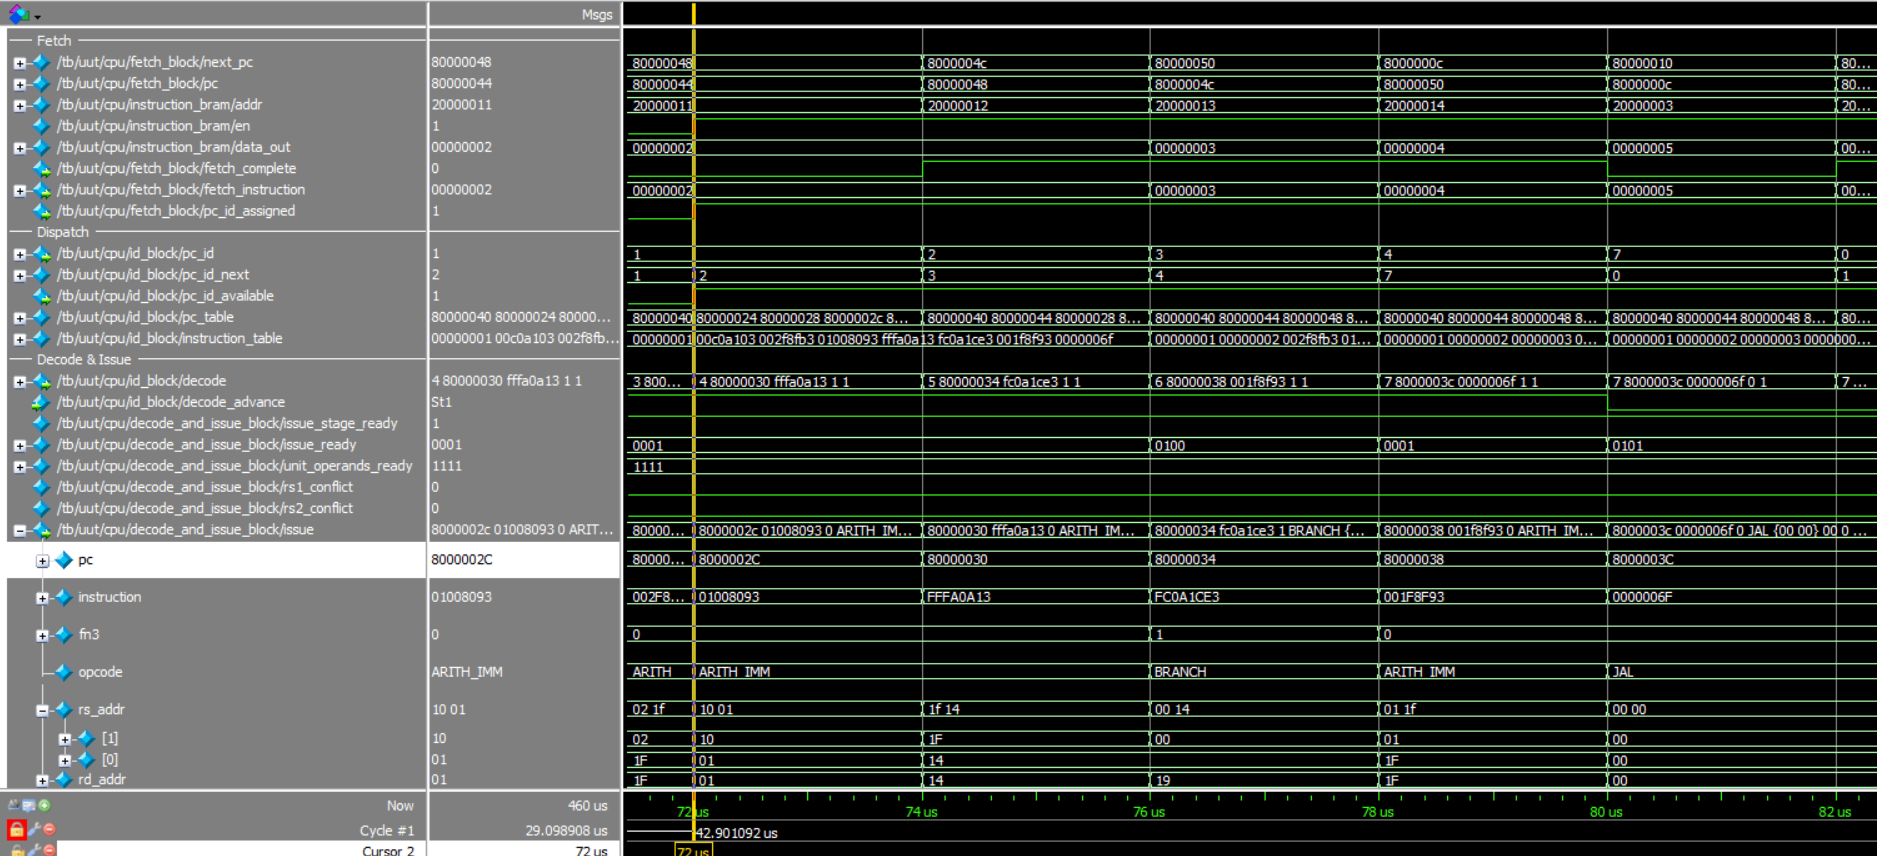
\includegraphics[width=1\linewidth]{../images/task3_8000002c}
	\caption{Временная диаграмма выполнения стадий декодирования и планирования на выполнение}
	\label{fig:task38000002c}
\end{figure}

Скриншот, полученный в ходе выполнения задания №4 (получить снимок экрана, содержащий временную диаграмму выполнения стадии выполнения команды с адресом 80000014 на первой итерации) представлен на рисунке \ref{fig:task480000014}.

\begin{figure}
	\centering
	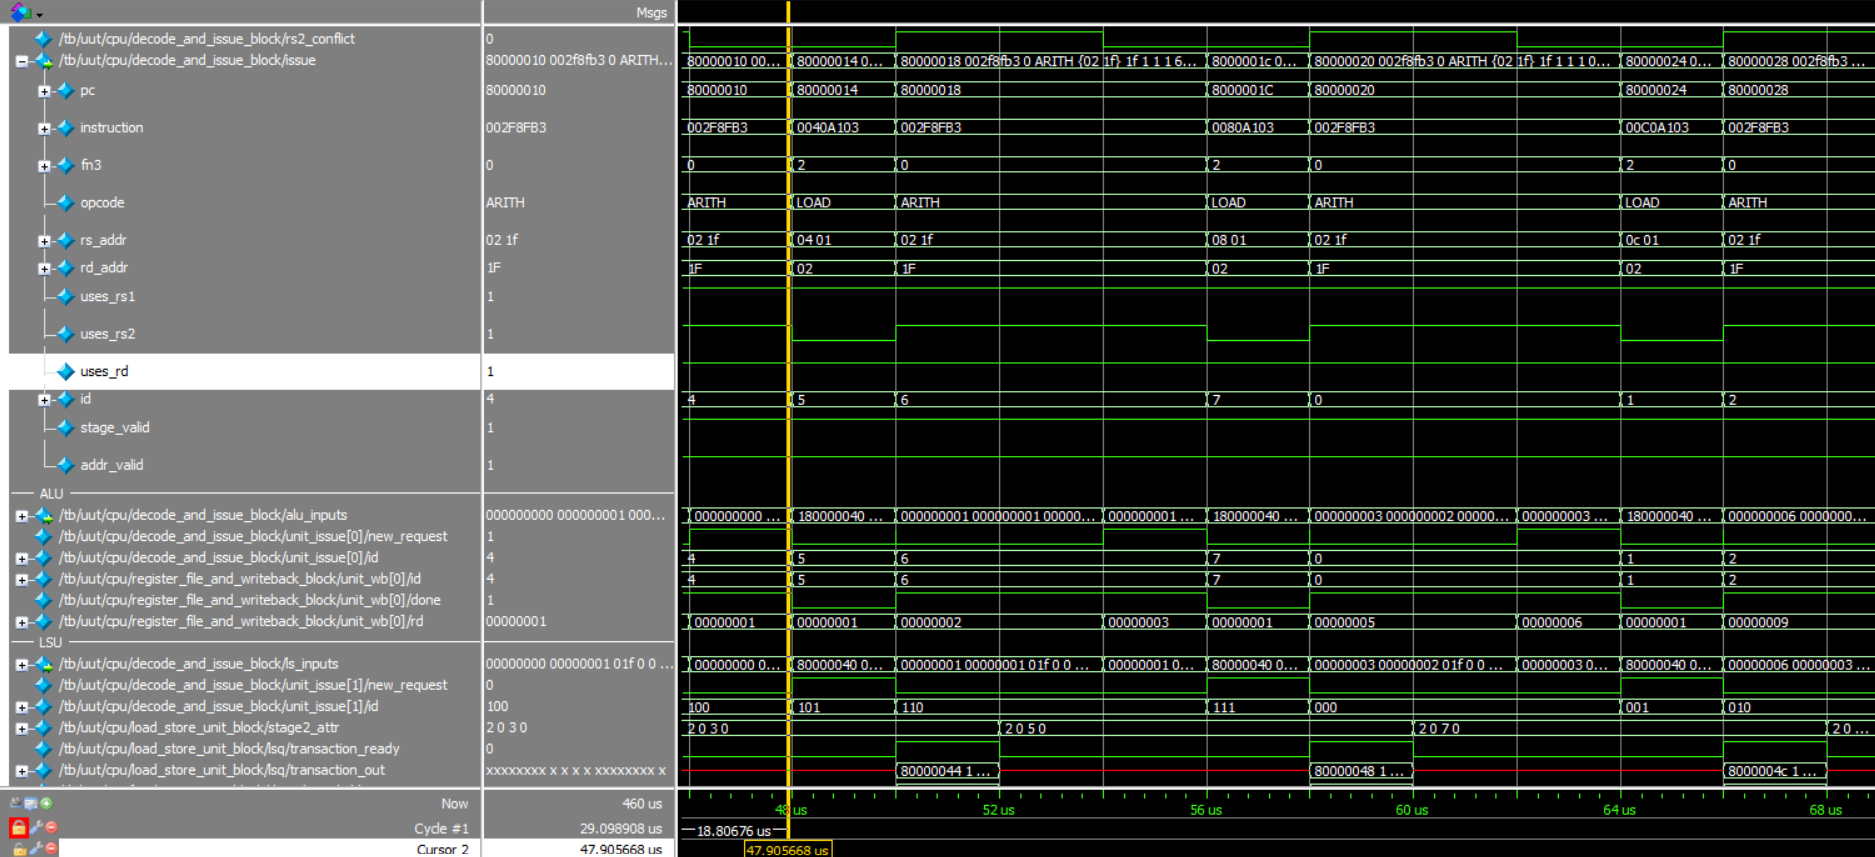
\includegraphics[width=1\linewidth]{../images/task4_80000014}
	\caption{Временная диаграмма выполнения стадии выполнения}
	\label{fig:task480000014}
\end{figure}

\section{Программа по варианту}

Все задания выполнялись по индивидуальному варианту №6.
Исходный текст исследуемой программы представлен на листинге \ref{lst:individual_s}.
\begin{lstinputlisting}[
	label={lst:individual_s},
	caption={Исходный текст индивидуальной программы},
	]{../riscv-lab/src/individual.s}
\end{lstinputlisting}
\newpage

Код программы на языке С, соответствующей индивидуальному варианту, представлен на листинге \ref{lst:individual_c}.
\begin{lstinputlisting}[
	label={lst:individual_c},
	language=C,
	caption={Код программы на языке С},
	]{../riscv-lab/src/individual.c}
\end{lstinputlisting}
\newpage	

\subsection{Трасса работы программы}

Трасса работы программы индивидуального варианта представлена на рисунке \ref{fig:individualpipeline}.

\begin{figure}
	\centering
	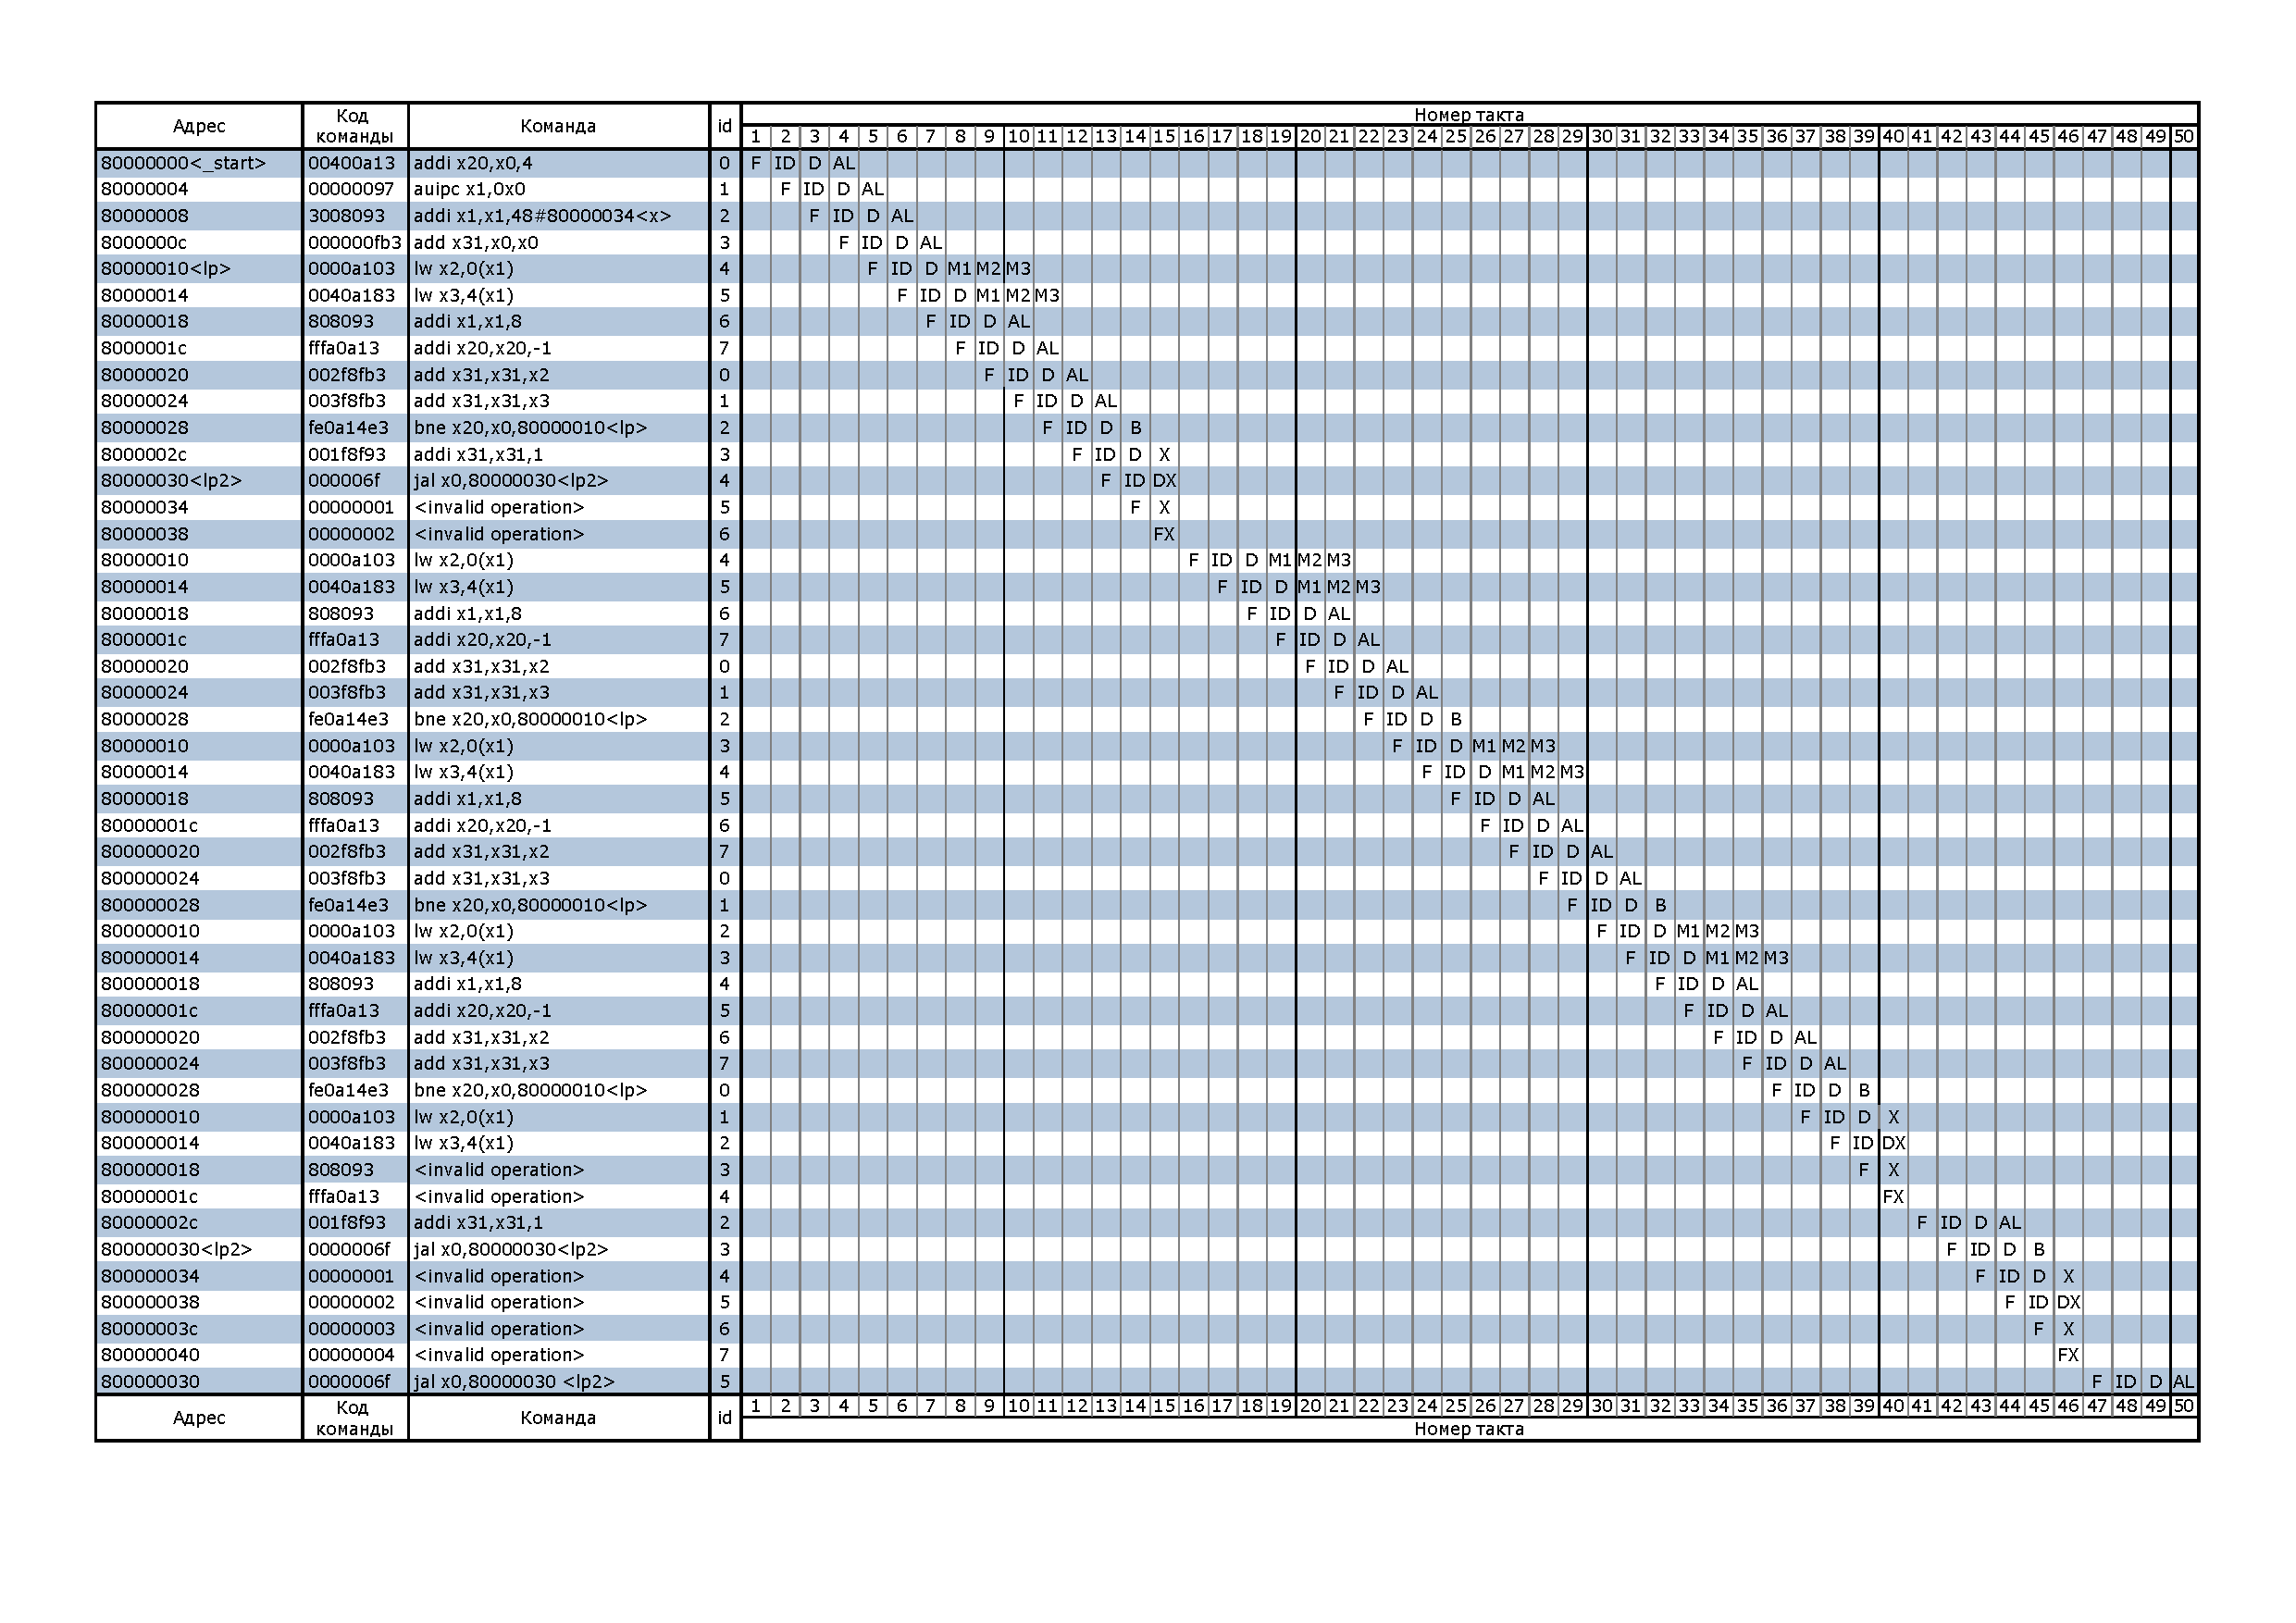
\includegraphics[width=1\linewidth]{../images/individual_pipeline}
	\caption{}
	\label{fig:individualpipeline}
\end{figure}


\subsection{Сравнение значения регистров}

Значение регистра x31 на момент окончания выполнения программы равно значению того же регистра, полученного в Задании №1, и равняется 25.

\begin{figure}
	\centering
	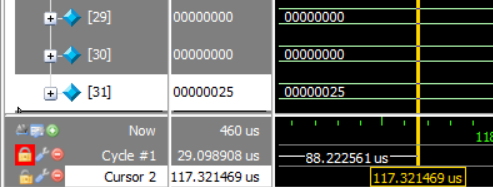
\includegraphics[width=0.5\linewidth]{../images/task5_01}
	\caption{Значение регистра x31 на момент окончания выполнения программы}
	\label{fig:task501}
\end{figure}


\subsection{Временные диаграммы сигналов}
Временные диаграммы сигналов, соответствующих всем стадиям выполнения команды, обозначенной в тексте программы символом \#! {lw x3, 4(x1)}, представлены на рисунке \ref{fig:task502}.
\begin{figure}
	\centering
	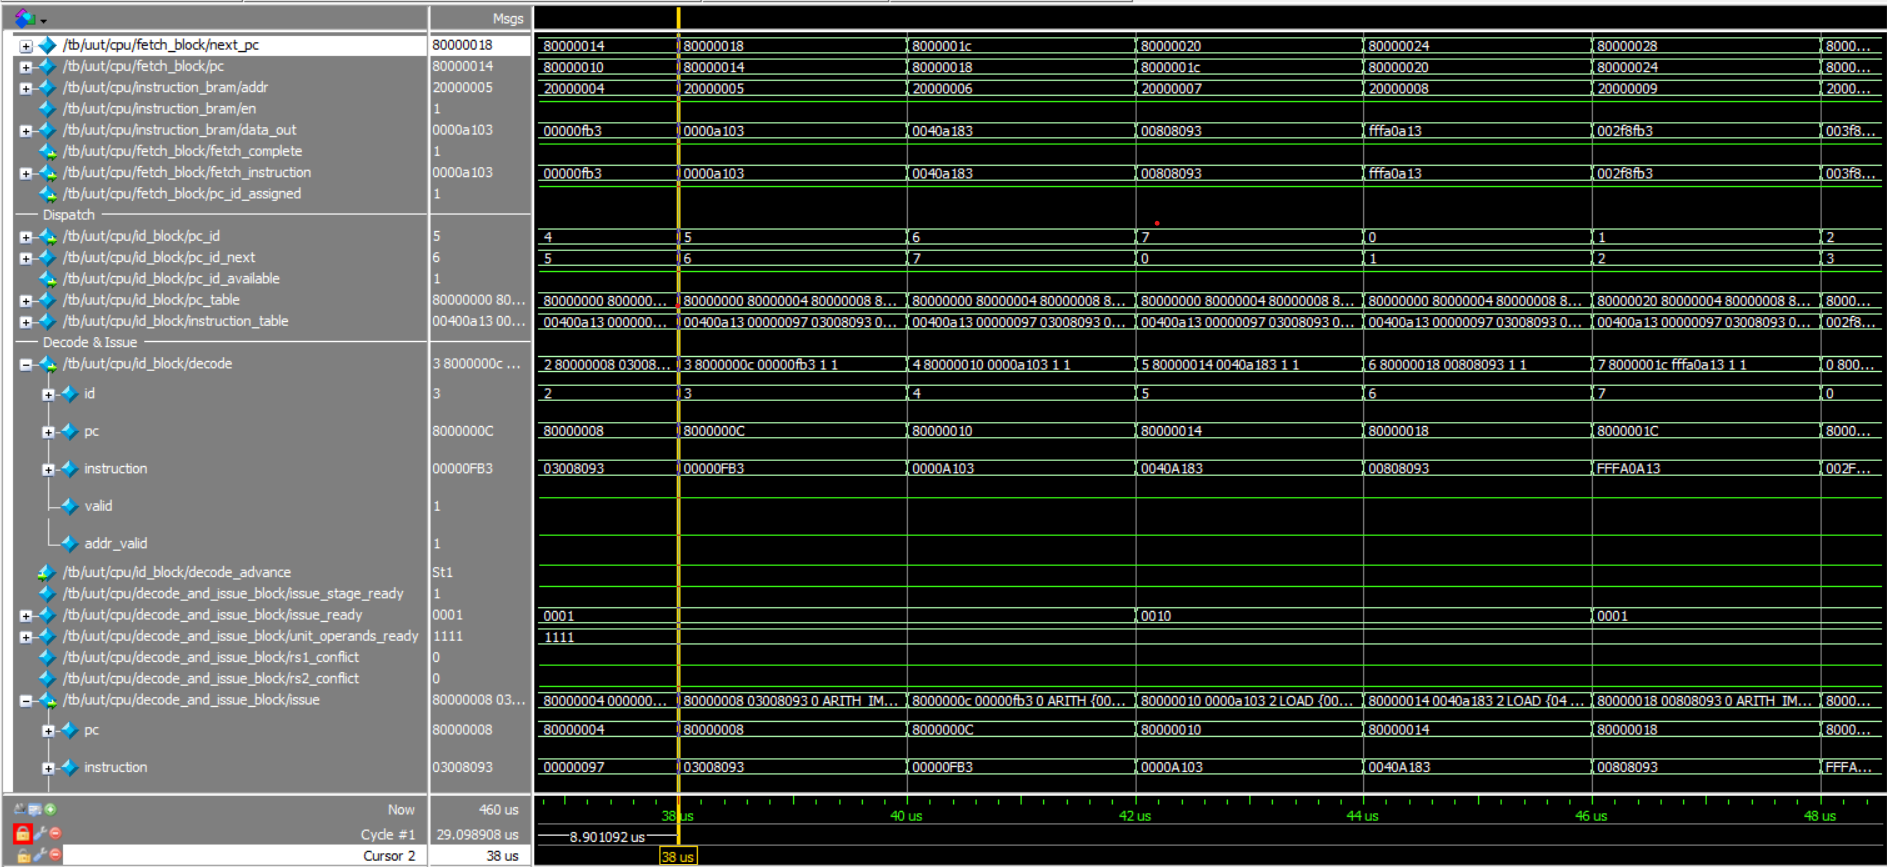
\includegraphics[width=1\linewidth]{../images/task5_02}
	\caption{Стадии выполнения команды lw x3, 4(x1)}
	\label{fig:task502}
\end{figure}

\section{Вывод об эффективности работы программы}
Как показано в ходе работы программы, представленной на рисунке \ref{fig:individualtrace}, не возникает никаких конфликтов, связанных с регистрами. 
Все команды выполняются немедленно после завершения предыдущей команды, благодаря грамотному распределению операций между операциями доступа к памяти и арифметическими операциями.
